\hypertarget{plaquette_8cpp}{}\section{plaquette.\+cpp File Reference}
\label{plaquette_8cpp}\index{plaquette.\+cpp@{plaquette.\+cpp}}


Details of the plaquette observable class (old)  


{\ttfamily \#include \char`\"{}Observables/plaquette.\+h\char`\"{}}\\*
{\ttfamily \#include \char`\"{}Observables/observable.\+h\char`\"{}}\\*
{\ttfamily \#include \char`\"{}Math/su3.\+h\char`\"{}}\\*
{\ttfamily \#include \char`\"{}Parallel\+Tools/parallel.\+h\char`\"{}}\\*
{\ttfamily \#include \char`\"{}Math/lattice.\+h\char`\"{}}\\*
{\ttfamily \#include $<$cstdio$>$}\\*
{\ttfamily \#include $<$cmath$>$}\\*
{\ttfamily \#include $<$string$>$}\\*
{\ttfamily \#include $<$iostream$>$}\\*
Include dependency graph for plaquette.\+cpp\+:\nopagebreak
\begin{figure}[H]
\begin{center}
\leavevmode
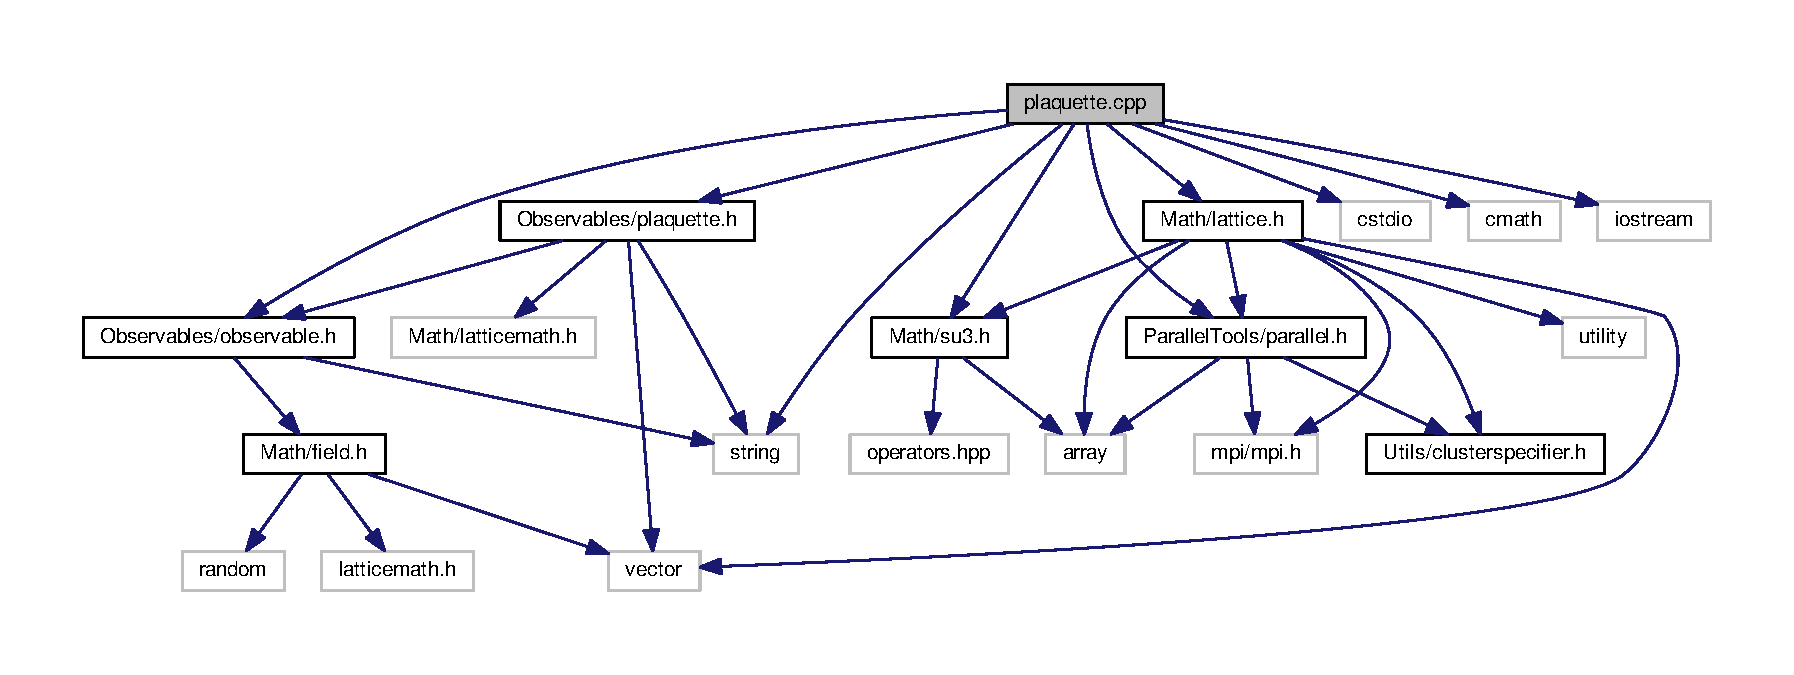
\includegraphics[width=350pt]{dc/dbf/plaquette_8cpp__incl}
\end{center}
\end{figure}


\subsection{Detailed Description}
Details of the plaquette observable class (old) 

\begin{DoxyAuthor}{Author}
Giovanni Pederiva 
\end{DoxyAuthor}
\begin{DoxyVersion}{Version}
0.\+1 
\end{DoxyVersion}
\begin{DoxyDate}{Date}
2017-\/2018 
\end{DoxyDate}
\begin{DoxyCopyright}{Copyright}
M\+IT License. 
\end{DoxyCopyright}
